% it/figures/literature/sterman_figures.tex — versione italiana
\begin{figure}[htbp]
    \centering
    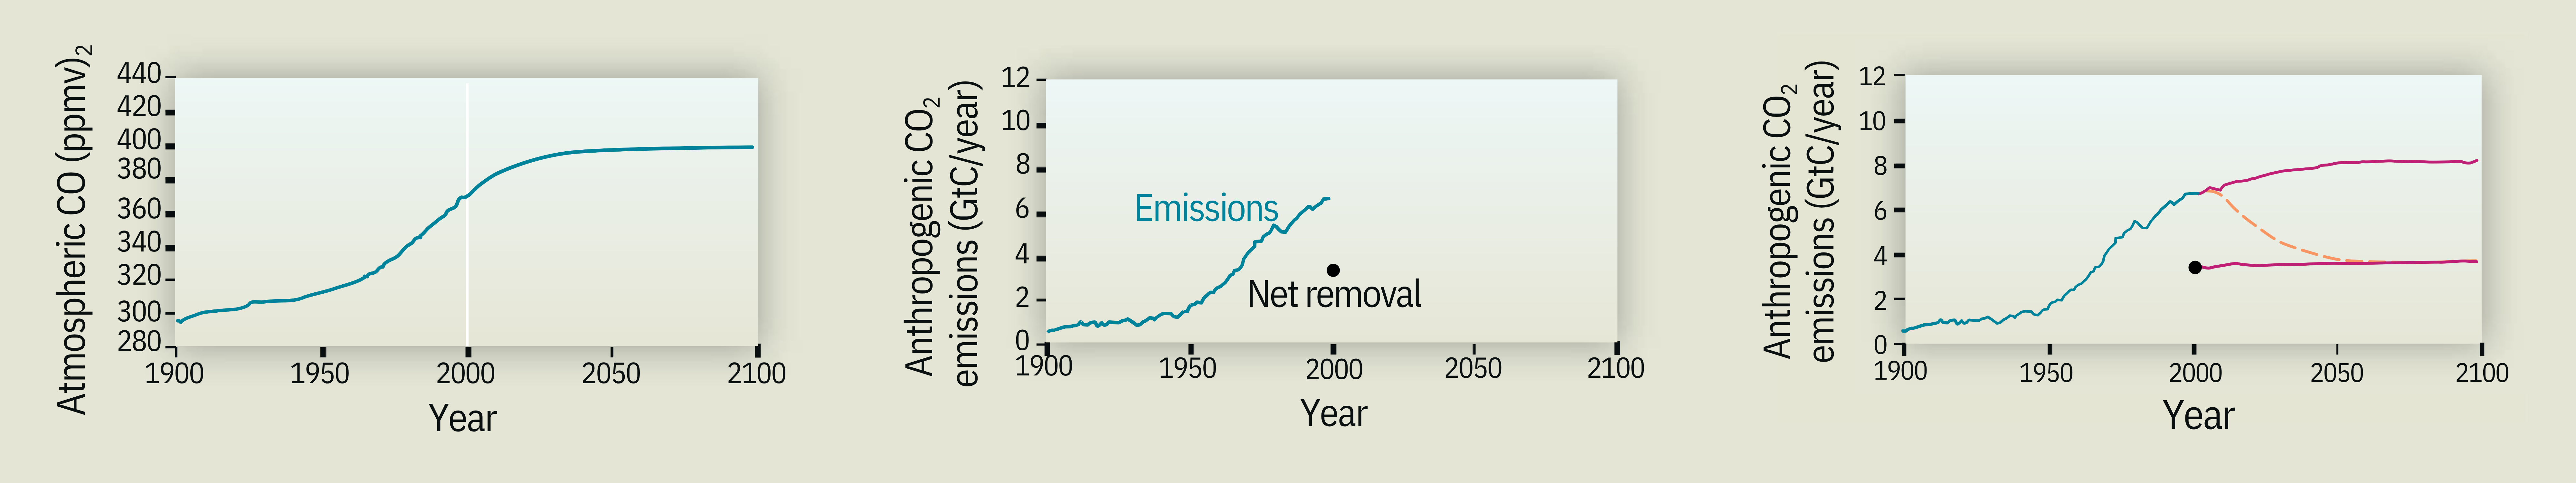
\includegraphics[width=\textwidth]{figures/literature/sterman_panel.png}
    \caption[Il compito di stabilizzazione del clima]{Il compito di stabilizzazione
    del clima. (a)~Lo scenario presentato ai partecipanti: la concentrazione
    atmosferica di CO\textsubscript{2} sale gradualmente a 400~ppmv e si stabilizza
    entro il 2100. (b)~L'informazione stock--flusso fornita: le emissioni antropiche
    di CO\textsubscript{2} dal 1900 al 2000 (il flusso in entrata) e l'attuale
    rimozione netta da parte di oceani e biomassa (il flusso in uscita), con le
    emissioni circa doppie rispetto alla rimozione netta. (c)~Una risposta tipica: i
    partecipanti disegnano erroneamente emissioni future che ricalcano la forma della
    traiettoria della CO\textsubscript{2} (euristica del pattern-matching), mentre il
    bilancio di massa richiede che le emissioni calino finché non eguagliano la
    rimozione netta (linea tratteggiata). Ristampato da \citet{sterman2008}.}
    \label{fig:sterman-panel}
\end{figure}
